% Offizielle Beispieldatei für beamer-Vorlage aus tubslatex Version 0.3beta2
\documentclass[fleqn,11pt,aspectratio=43]{beamer}

\usepackage[ngerman]{babel}
\usepackage[utf8x]{inputenc}
\usepackage{svg}
\usepackage{graphicx}
\usetheme[%
  %nexus,%        Nexus Fonts benutzen
  %lnum,%         Versalziffern verwenden
  %cmyk,%<rgbprint>,          Auswahl des Farbmodells
  blue,%<orange/green/violet> Auswahl des Sekundärfarbklangs
  dark,%<light,medium>        Auswahl der Helligkeit
  %colorhead,%    Farbig hinterlegte Kopfleiste
  %colorfoot,%    Farbig hinterlegt Fußleiste auf Titelseite
  colorblocks,%   Blöcke Farbig hinterlegen
  %nopagenum,%    Keine Seitennumer in Fußzeile
  %nodate,%       Kein Datum in Fußleiste
  tocinheader,%   Inhaltsverzeichnis in Kopfleiste
  %tinytocinheader,% kleines Kopfleisten-Inhaltsverzeichnis
  %widetoc,%      breites Kopfleisten-Inhaltsverzeichnis
  %narrowtoc,%    schmales Kopfleisten-Inhaltsverzeichnis
  %nosubsectionsinheader,%  Keine subsections im Kopfleisten-Inhaltsverzeichnis
  %nologoinfoot,% Kein Logo im Fußbereich darstellen
  ]{tubs}

% Titelseite
\title{Entwicklung Adaptiver Regler}
\subtitle{für Kälte}
\author{Carl Julius Martensen}
% Titelgrafik, automatisch beschnitten, Weitere Optionen: <scaled/cropx/cropy>
% \titlegraphic[cropped]{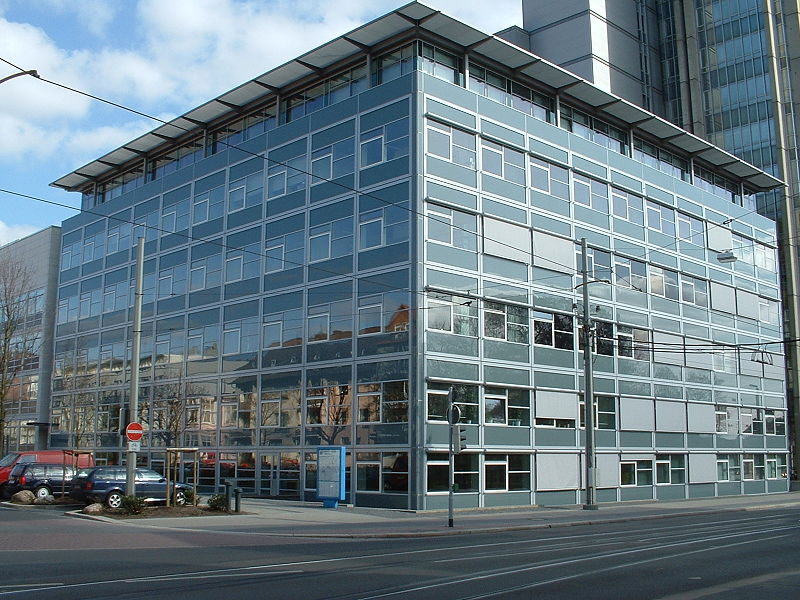
\includegraphics{infozentrum.jpg}}
\titlegraphic[scaled]{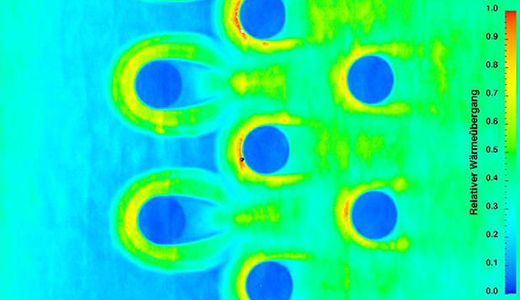
\includegraphics{Titelbild}}

% Logo, dass auf Titelseiten oben rechts und auf Inthaltsseiten unten rechts
% dargestellt wird. Es wird jeweils automatisch skliert
\logo{
\includegraphics{ift_4C.pdf}}
%\logo{Institut für Unkreativität\\und Schreibschwäche}

\begin{document}

\begin{frame}[plain]
\titlepage
\end{frame}

\section{Vorgehensweise}

\begin{frame}{Zeitleiste}

\begin{figure}
\includesvg[width = \linewidth]{control_standard}
\end{figure}

\end{frame}

\begin{frame}{Zeitleiste}

\begin{figure}
\includesvg[width = \linewidth]{Kreislauf}
\end{figure}

\end{frame}

\begin{frame}{Zeitleiste}

Hier einmal die Tools vorstellen

\end{frame}

\begin{frame}
Regelgüte erläutern
\end{frame}

\begin{frame}

Stabilität:

Was ist stabilität?
Praktisches Beispiel

Bilder aus dem Phasendiagramm

Robustheit

Was ist robustheit?
Nyquistkurve!
Sensitivität!

\end{frame}

\begin{frame}
Modellidentifizierung
Warum?
Wie?
Beispiele -> Nyquist, Bodeplot
\end{frame}

\begin{frame}
Robustheit in Zusammenhang mit Identifizierung!
\end{frame}

\begin{frame}{Zeitleiste}

\begin{figure}
\includesvg{../Graphics/SISO_Robustness_Study}
\end{figure}

\end{frame}

\begin{frame}
Störungen durch Kopplung!
-> Beeinflussen Stabilität und Regelgüte!
-> Beeinflussen damit auch Performance!
\end{frame}

\begin{frame}
Idee: Verbessern durch Modellmehrwert
Kopplungen mitmessen, dadurch vorhersage von verhalten möglich!
\end{frame}

\begin{frame}
Systemauslegung:

Features:

Vorteile:

\end{frame}

\end{document}
